\chapter{Systems Development}

\section{Introduction}
Creating good software requires good coding skills, so you can get the computer to do what you want. Additionally, however, it requires good "systems development" skills so that (1) your code is organized / quickly updateable by yourself and others and (2) designing the product your users want, rather than what you \emph{think} they want. Systems development is a useful concept not just for computer science projects, but for any type of product development. 

For code organization, we use \textbf{APIs}, which are a set of functions and procedures to allow different portions of code in a big project to communicate with each other. For user-guided product design, we use \textbf{iterative design}, which is the process of making many imperfect iterations of a project to prototype on users before trying to make the final product. 

\section{Code Organization}

 \subsection{Modularity}
 \textbf{Modularity} means that code can be separated into many smaller components that are relatively independent. 
 
Modularity has two primary benefits:
\begin{itemize}
\item It allows different people to work on different portions of the code without interfering with one another. This is how software companies like Google, Amazon, and Microsoft can have tens of thousands of teammembers all working on the same project.
\item It ensures that if one portion of the code needs to be updated or fixed, the rest of the code will not be impacted. 
\end{itemize} 

To illustrate this, we will consider modularity's usefulness in cars. Cars are incredibly complicated, but they can be understood by considering them as a collection of components. Each component has its own functionality. 

A few components of a car include:
\begin{itemize}
\item Tires: a round object that can attach to an axle
\item Engine: a device that can spin an axle
\item Axle: a rod that can be connected in the center to an engine, and at the edges to tires
\end{itemize} 

There are different ways to design each of these. They can each be made from a number of materials, and there are different varieties and sizes of each (e.g. 4 vs 6 cylinder engine, snow vs all-season tire, etc.). Furthermore, any \textit{combination} of these different varieties can be put together: we can change the type of tires we have without thinking about what type of axle or motor is in the car. 

The first thing to note is that car companies can now divide up labor in multiple teams, and those teams won't interfere with each other as they work. One team can spend months developing the axle: finding the right alloy, shape, and weight to handle the load from the car, for example. Another team can spend months developing the engine: trying out different arrangements of the cylinders or different numbers of cylinders, for example. What's more, car manufacturers almost always outsource the production of their tires to tire manufacturers: they leave the decisions on the type of rubber and the proper shape to a team totally outside of their company. The modularity of the car allows these teams to work totally separately, with the only communication between them the above list: the tire must attach to an axle, the engine must spin the axle, and the axle must connect to the engine and the tires. Once the teams agree on the way they will bolt the systems together, they no longer have to communicate. 

The second thing to note is that modularity allows car enthusiasts to upgrade and customize their vehicles without having to redesign the whole thing. If a vehicle owner wants to replace their V6 with a V8, they can do that as long as the connections between the motor and the rest of the vehicle are the same (i.e. the connection to the axle, to the fuel source, etc). If a vehicle owner wants to replace their all season tires for snow tires in the winter, they can do that as long as the connection with the rest of the vehicle is the same (i.e. the connection to the axle is the same). 

\subsection{APIs}
An \textbf{API}, or Application Programming Interface, is a list of components in a system, and the basic functionality of each of the components. The list of car components above is one example of an API: it describes the objects in a car, and what each of them is expected to do. As we saw in the previous section, this acts as a "contract" between different teams working on a project to ensure that they can work independently: as the axle-maker, I don't know what kind of tire the other team will come up with, all I know is the way I am expected to make my axle attach to the tire. 

We will know come back to coding to consider an example of an API for a simple software project. \todo{What should I use as an example} 

\subsection{Example}
Make the API for an ATM

%\begin{figure}
%	\centering
%	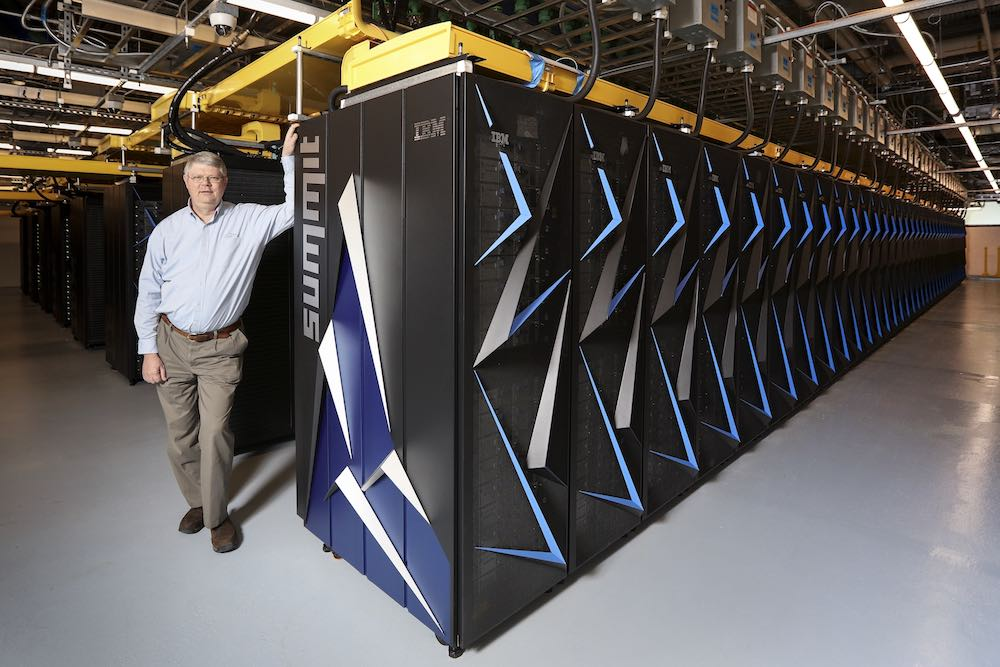
\includegraphics[width=0.85\textwidth]{images/supercomputer.jpg}
%	\caption{Summit, a world-class supercomputing cluster at Oak Ridge National Laboratory in Tennessee. Credit: https://insidehpc.com/2018/11/new-top500-list-lead-doe-supercomputers/}
%	\label{fig:supercomputer}
%\end{figure}

\section{User-oriented Design}

\subsection{Activity}
Spaghetti, tape, and some floral foam (?) 

\subsection{Example}
Drawing an owl

\subsection{Iteration design}
Talk about the waterfall method in contrast to iterative design. Goal is to get feedback. Fail fast / get minimum viable product out there because you might find out you need a totally new product before you realize 

\subsection{Hierarchical design}
Start with big picture -- that's how you draw an owl. Start with the most important ideas first. 

\section{Summary}


\referencessection

Computer Science: An Interdisciplinary Approach, Robert Sedgewick and Kevin Wayne.

University of Wisconsin-Madison CS 202 Lectures, Andrea Arpaci-Dusseau. (http://pages.cs.wisc.edu/~dusseau/Classes/CS202-F11/)
